\section{Week 7}
\begin{table}[H]
\centering
\begin{tabular}{|c|c|c|}
\hline
                 & \textbf{Incompressible Flow} & \textbf{Compressible Flow} \\ \hline
\textbf{\begin{tabular}[c]{@{}c@{}}Kinetic\\ Energy\end{tabular}}        & low   & High  \\ \hline
\textbf{Density} & constant                     & Varing                     \\ \hline
\textbf{\begin{tabular}[c]{@{}c@{}}Temperature\\ Variation\end{tabular}} & small & Large \\ \hline
\end{tabular}
\end{table}

\Large \textbf{\underline{Governing Equations}}

\begin{itemize}
    \item \color{blue} \textbf{Conservation of Mass / Continuity} \color{black}
    \begin{equation*}
        \rho_1 A_1 U_1 = \rho_2 A_2 U_2
    \end{equation*}
    \item \color{blue} \textbf{Conservation of Momentum} \color{black}
    \begin{equation*}
        -\rho_1 A_1 U_1^2 + \rho_2 A_2 U_2^2 = P_1 A_1 - P_2 A_2 
    \end{equation*}
    \item \color{blue} \textbf{Conservation of Energy} \color{black}
    \begin{align*}
        \frac{P_1}{\rho_1} + e_1 + \frac{U_1^2}{2} &= \frac{P_2}{\rho_2} + e_2 + \frac{U_2^2}{2} \\
        h_1 + \frac{U_1^2}{2} &= h_2 + \frac{U_2^2}{2}
    \end{align*}
    \textbf{\underline{Internal energy}} $e$ is the sum of energies of all molecules of a gas.
    \item \color{blue} \textbf{Equation of State} \color{black}
    \begin{align*}
        P &= \rho R T \\
        \text{where } R_{\text{air}} &= 287 \, \text{J/kg$^{-1}$K$^{-1}$} \\
        R_{\text{gas}} &= \frac{R_u\, [\text{J/K$\cdot$mol}]}{M\,[\text{kg/mol}]} = \frac{8.314}{M}
    \end{align*}
    \item Others
    \begin{align*}
        R &= c_p - c_v \\
        \gamma &= \frac{c_p}{c_V} \\
        c_p &= \frac{\gamma R}{\gamma - 1} \\
        c_v &= \frac{R}{\gamma - 1} \\
        u &= m c_v T
    \end{align*}
    where $c_p$ and $c_v$ are specific heat constants at constant pressure and at constant volume [J/kg$\cdot$K], $\gamma$ is the isentropic expansion factor, $\gamma = 1.4$ for air and $\gamma = 1.33$ for $\text{CO}_2$.
    
    \item Equipartition of Energy
    \begin{itemize}
        \item Internal energy ($u$) of a gas is equally distributed among each DoF: $u = \frac{1}{2} RT$ per DoF.
        \item Monatomic gases has 3 translational DoF and 0 rotational DoF.
    \end{itemize}
\end{itemize}

\Large \textbf{\underline{\color{red}Enthalpy\color{black}}}
\vspace{5mm}

Enthalpy is the sum of internal energy and a pressure-volume (work) term:
\begin{align*}
    h &= \text{internal energy} + \text{work term} \\
    h &= e + pv \\
    h &= e + \frac{P}{\rho}
\end{align*}
($v$ is specific volume, $v=1/\rho$)

\begin{itemize}
    \item For a perfect gas:
    \begin{align*}
        e = f(T) &= c_v \, T \\
        h = f(T) &= c_p \, T \\
        (h_2 - h_1) &= c_p (T_2 - T_1) 
    \end{align*}
    \begin{itemize}
        \item For a calorically perfect gas, $c_v$ and $c_p$ are constant (holds for $T< 1000 K$)
    \end{itemize}
\end{itemize}

\vspace{5mm}

\Large \textbf{\underline{\color{red}Entropy\color{black}}}

\begin{itemize}
    \item Reversible Process: $ds = \frac{\partial q}{T} + \color{red}\cancel{ds_{irrev}}$\color{black}
    \begin{itemize}
        \item one in which no dissipative phenomena occur
        \item not a good assumption near surfaces / sudden change in properties (shocks)
    \end{itemize}
    \item Adiabatic process: $ds = \color{red}\cancel{\frac{\partial q}{T}}\color{black}+ds_{irrev}$
    \begin{itemize}
        \item one in which no heat is added or taken away from the system
        \item not a good assumption in combustion problems
        \item valid in shocks
    \end{itemize}
    \item \textbf{Isentropic process} ($ds=0$)
    \begin{align*}
        \frac{P_2}{P_1} &= \left(\frac{\rho_2}{\rho_1}\right)^{\gamma} = \left(\frac{T_2}{T_1}\right)^{\frac{\gamma}{\gamma-1}} \\
        \frac{P}{\rho} &= \text{const}
    \end{align*}
    \item \textbf{Non-isentropic process}
    \begin{align*}
        s_2 - s_1 &= c_p \ln\left(\frac{T_2}{T_1}\right) - R \ln\left(\frac{P_2}{P_1}\right) \\
        &= c_v \ln\left(\frac{T_2}{T_1}\right)+ R \ln\left(\frac{V_2}{V_1}\right)
    \end{align*}
\end{itemize}

\Large \textbf{\underline{\color{blue}Compressibility Criteria\color{black}}}

\begin{itemize}
    \item A flow is considered compressible if
    \begin{align*}
        v &> 0.30 a \\
        \text{where } a^2 &= \gamma \cdot \frac{P}{\rho} = \gamma R T \\
        a^2 &= \frac{dP}{d\rho}
    \end{align*}
\end{itemize}

\Large \textbf{\underline{\color{blue}Mach Number\color{black}}}

\begin{itemize}
    \item Definition:
    \begin{equation*}
        M = \frac{V}{a}
    \end{equation*}
    \begin{align*}
        \text{if } M &> 1 \to \text{ supersonic flow} \\
        \text{if } M &> 0.3 \to \text{ compressibility criteria} \\
        \text{if } M &< 1 \to \text{ subsonic flow} \\
        \text{if } M &= 1 \to \text{ sonic flow} \\
    \end{align*}
    \item Mach Angle
    \begin{equation*}
        \sin(\mu) = \frac{a\cdot t}{ M \cdot a \cdot t} = \frac{1}{M}
    \end{equation*}
\end{itemize}

\Large \textbf{\underline{\color{blue}Stagnation Summary\color{black}}}
\vspace{3mm}

The general formula:
\begin{equation*}
    \frac{\chi_0}{\chi} = f(M)\,\text{for a given gas with } \gamma
\end{equation*}

Stagnation conditions are identical for isentropic processes.

\begin{itemize}
    \item \textbf{Stagnation Temperature} \color{green}(adiabatic flow)\color{black}
    \begin{equation*}
        \frac{T_0}{T} = 1+ \frac{\gamma - 1}{2} M^2
    \end{equation*}
    \item \textbf{Stagnation Pressure} \color{green}(Isentropic flow) \color{black}
    \begin{equation*}
        \frac{P_0}{P} = \left(1+\frac{\gamma - 1}{2} M^2\right)^{\frac{\gamma}{\gamma-1}}
    \end{equation*}
    \item \textbf{Stagnation Density} \color{green}(Isentropic flow)\color{black}
    \begin{equation*}
        \frac{\rho_0}{\rho} = \left(1+\frac{\gamma-1}{2}M^2\right)^{\frac{1}{\gamma-1}}
    \end{equation*}
    \item Don't use the above equations. Use \href{http://www.dept.aoe.vt.edu/\~devenpor/aoe3114/calc.html}{\color{blue}\underline{Online Calculator}\color{black}}.
\end{itemize}

\Large \textbf{\underline{\color{blue}Flow Nozzles\color{black}}}
\vspace{3mm}

\begin{itemize}
    \item Conservation of momentum
    \begin{equation*}
        -\frac{dP}{\rho V^2} = \frac{d\rho}{\rho} + \frac{dA}{A} + 2 \cdot \frac{dV}{V}
    \end{equation*}
    \item Conservation of mass
    \begin{equation*}
        0 = \frac{d\rho}{\rho} + \frac{dA}{A} + \frac{dV}{V}
    \end{equation*}
    \item Algebraic manipulations (describes what happens in compressible flow nozzles):
    \begin{itemize}
        \item Density / Velocity Rule
        \begin{align*}
            \frac{d\rho}{\rho} &= - M^2 \cdot \frac{dV}{V} \\
            \text{introduces } M &= \frac{V}{a}
        \end{align*}
        \item Area-velocity Rule:
        \begin{align*}
            \frac{dA}{A} &= (M^2 - 1) \cdot \frac{dV}{V}
        \end{align*}
    \end{itemize}
\end{itemize}

\Large \textbf{\underline{\color{red}Area-Velocity Rule in different cases:\color{black}}}
\vspace{3mm}
\begin{itemize}
    \item $M=0$ (\color{blue}incompressible flow\color{black})
    \begin{equation*}
        \frac{dA}{A} = - \frac{dV}{V}
    \end{equation*}
    Fraction {\color{blue} decrease in area } is {\color{blue} equal} to the fraction {\color{blue} increase in velocity}.
    \item $0< M < 1$ ({\color{blue}subsonic flow})
    \begin{equation*}
        \frac{dA}{A} \propto - \frac{dV}{V}
    \end{equation*}
    Fraction {\color{blue} decrease in area } is {\color{blue} proportional} to the fraction {\color{blue} increase in velocity}.
    \begin{figure}[H]
        \centering
        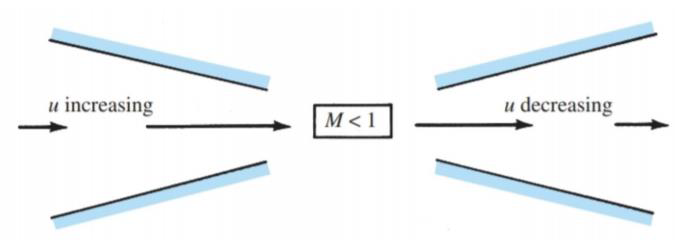
\includegraphics[width=1.0\linewidth]{images/area_velocity_subsonic_flow.png}
    \end{figure}
    \item $M=1$ ({\color{blue}sonic flow})
    \begin{equation*}
        \frac{dA}{A} = 0
    \end{equation*}
    No change in area. Sonic conditions will only be met at {\color{blue}minima or throat} of the nozzle.
    \item $M>1$ ({\color{blue}supersonic flow})
    \begin{equation*}
        \frac{dA}{A} \propto \frac{dV}{V}
    \end{equation*}
    Fraction {\color{blue} increase in area } leads to fraction {\color{blue} increase in velocity}.
    \begin{figure}[H]
        \centering
        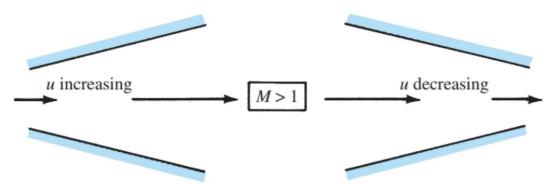
\includegraphics[width=1.0\linewidth]{images/area_velocity_supersonic_flow.png}
    \end{figure}
\end{itemize}

\textbf{Problem:} We can never get supersonic flow with only a converging nozzle.

\textbf{Why?} Because when you continually decrease area, {\color{blue}velocity V goes up}, but {\color{red}desntiy $\rho$ goes down due to $\frac{d\rho}{\rho}\propto - \frac{dV}{V}$}. Then, the speed of sound increases due to $a^2 = \gamma \frac{P}{\rho}$.

\textbf{Solution:}
\begin{itemize}
    \item to achieve supersonic flow $\rightarrow$ must have a convergent-divergent nozzle.
    \begin{enumerate}
        \item {\color{blue}Convergent nozzle} to accelerate subsonic flow
        \item Sonic conditions at {\color{blue} throat}
        \item {\color{blue}Divergent nozzle} to accelerate beyond $M>1$
    \end{enumerate}
    \begin{figure}[H]
        \centering
        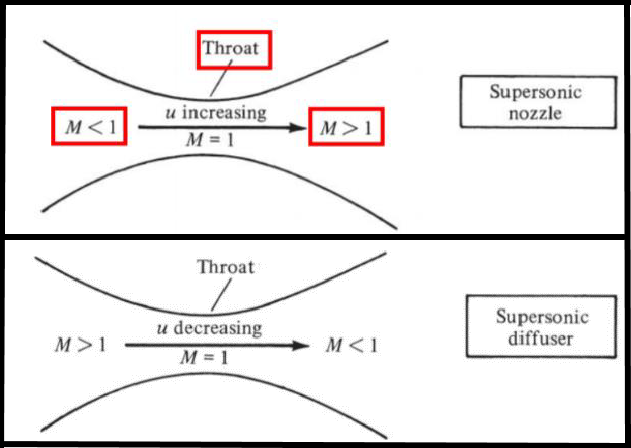
\includegraphics[width=1.0\linewidth]{images/supersonic_nozzle_diffuser.png}
    \end{figure}
\end{itemize}

\Large \textbf{\underline{\color{blue}Air-Mach Relation\color{black}}}
\vspace{3mm}

\begin{figure}[H]
    \centering
    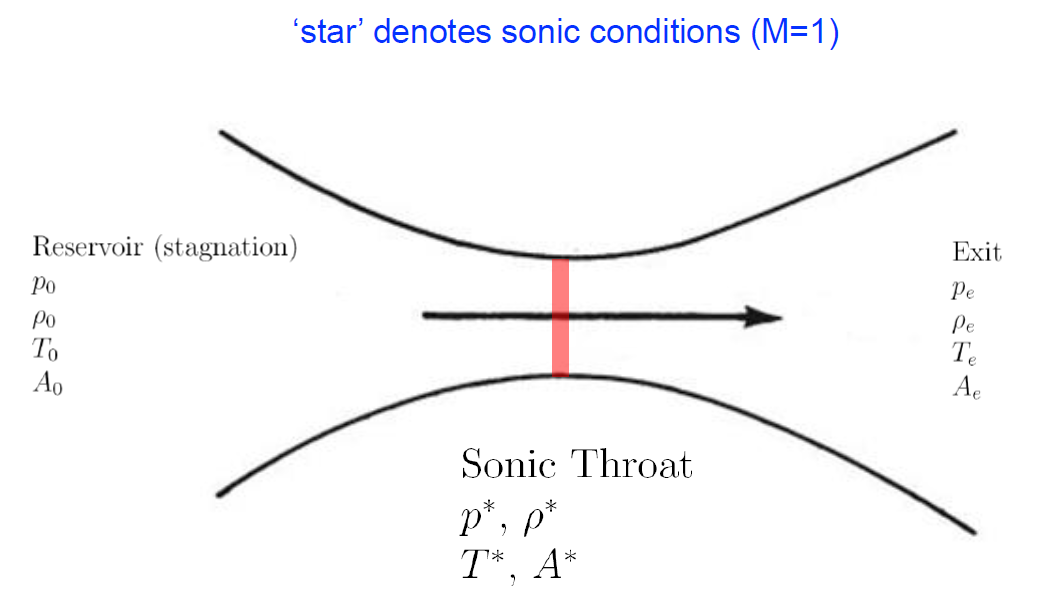
\includegraphics[width=1.0\linewidth]{images/throat.png}
\end{figure}
\begin{equation*}
    \left(\frac{A}{A^*}\right)^2 = \frac{1}{M^2}\left[\frac{2}{\gamma+1}\left(1+\frac{\gamma-1}{2}M^2\right)\right]^{\frac{\gamma+1}{\gamma-1}}
\end{equation*}
\begin{itemize}
    \item For any value of $\frac{A}{A^*}$ there are two values of $M$.
    \item Stagnation ratios, namely,
    \begin{align*}
        \frac{T_0}{T^*} &= 1.200 \, , \\
        \frac{P_0}{P^*} &= 1.893 \, , \\
        \frac{\rho_0}{\rho^*} &= 1.577 \, ,
    \end{align*}
    are fixed at the throat for any supersonic nozzle.
    \item {\color{red}Flow in nozzle is driven by pressure difference.}
\end{itemize}


